\documentclass[a4paper, 12pt]{report}
\usepackage[T2A]{fontenc}
\usepackage[english, russian]{babel}
\usepackage{graphicx}
\graphicspath{{./Images/}}
\usepackage[utf8]{inputenc}
\usepackage[backend=bibtex,bibencoding=utf8,sorting=nty,maxcitenames=2,style=numeric-comp]{biblatex}
\addbibresource{bibliography.bib}

\begin{document}
	\chapter{Атаки на сети уровня L2}
		\section{ARP-Spoofing}
		
		ARP-spoofing — разновидность сетевой атаки типа MITM, применяемая в сетях с использованием протокола ARP. В основном применяется в сетях Ethernet. Атака основана на недостатках протокола ARP.
		
		Злоумышленник выбирает машину или машины жертвы
		Первым шагом в планировании и реализации атаки ARP Spoofing является выбор цели. Это может быть конкретная конечная точка в сети, группа конечных точек или сетевое устройство, такое как маршрутизатор. Маршрутизаторы являются привлекательными целями, поскольку успешное отравление ARP маршрутизатора может нарушить трафик для всей подсети.
		Злоумышленник запускает инструменты и начинает атаку
		\begin{figure}[h!]
			\centering
			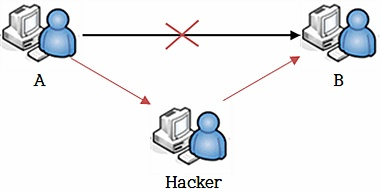
\includegraphics[scale=0.45]{img/2.jpg}
			\caption{MITM}
			\label{chargets}
		\end{figure}
		Всем злоумышленникам, желающим выполнить отравление ARP, легко доступен широкий спектр инструментов. После запуска выбранного инструмента и настройки соответствующих параметров злоумышленник начинает атаку. Он может незамедлительно начать рассылку сообщений ARP или дождаться получения запроса.
		Злоумышленник выполняет определенные действия с некорректно направленным трафиком
		После повреждения кэша ARP на устройстве (устройствах) жертвы злоумышленник обычно выполняет какие-то действия с некорректно направленным трафиком. Он может просматривать или изменять его, либо создать «черную дыру», чтобы данные никогда не доходили до адресата. Выбор действий зависит от мотивов злоумышленника.
		
	
\end{document}
